\section{Neural Networks as Function Approximators}
\label{ch1:sec3}

In this section we introduce artificial neural networks, usually called neural networks, which are computing systems inspired by the biological neural networks that constitute animal brains. It has been shown that these systems can be used very well as classifiers as well as regressors or function approximators. \\
These neural networks are based on simplified models of biological neurons, which are special cells within the nervous system which transmit information to other nerve, muscle, or gland cells. 

The connections of the biological neuron are modeled as
weights. A positive weight reflects an excitatory connection, while negative values mean
inhibitory connections. All inputs are modified by a weight and summed. This activity is
referred to as a linear combination. Finally, an activation function controls the amplitude of the
output.

An ANN is based on a collection of connected units or nodes called artificial neurons, which loosely model the neurons in a biological brain. Each connection, like the synapses in a biological brain, can transmit a signal to other neurons.

The "signal" at a connection is a real number, and the output of each neuron is computed by some non-linear function of the sum of its inputs.

The first mathematical model for a single neuron, termed the perceptron, was described in \cite{Rosenblatt:1958} and is still in use today. We want to use perceptrons and the neural networks constructed from them to generate function values (output) that approximate the values of the solution to our differential equation from data (input) that will be the domain of our differential equation. \\
We now describe how a perceptron transforms a reel-valued input into a one-dimensional output, as illustrated in \cref{fig4}. Let there be $n$ input values $x_1, \ldots, x_n \in \mathbb{R}$, which can be understood as the entries of a vector $x \in \mathbb{R}^n$. First one forms a biased linear combination with the input values, i.e. 
\begin{equation*}
    a = \sum^{n}_{i=1} w_i x_i + b = w^{\mathrm{T}} x + b,
\end{equation*}
where $w_1, \ldots, w_n \in \mathbb{R}$ are called weights and $b \in \mathbb{R}$ is called bias. In general, these weights are learned through an amount of data. Then an activation function $\sigma \colon \mathbb{R} \to \mathbb{R}$, which is non-linear, is applied to $a$, so that the output of the neuron becomes
\begin{equation*}
    z = \sigma(\sum^{n}_{i=1} w_i x_i + b) = \sigma(w^{\mathrm{T}} x + b) = \sigma(a).
\end{equation*}

\begin{figure}[H]
    \begin{center}
        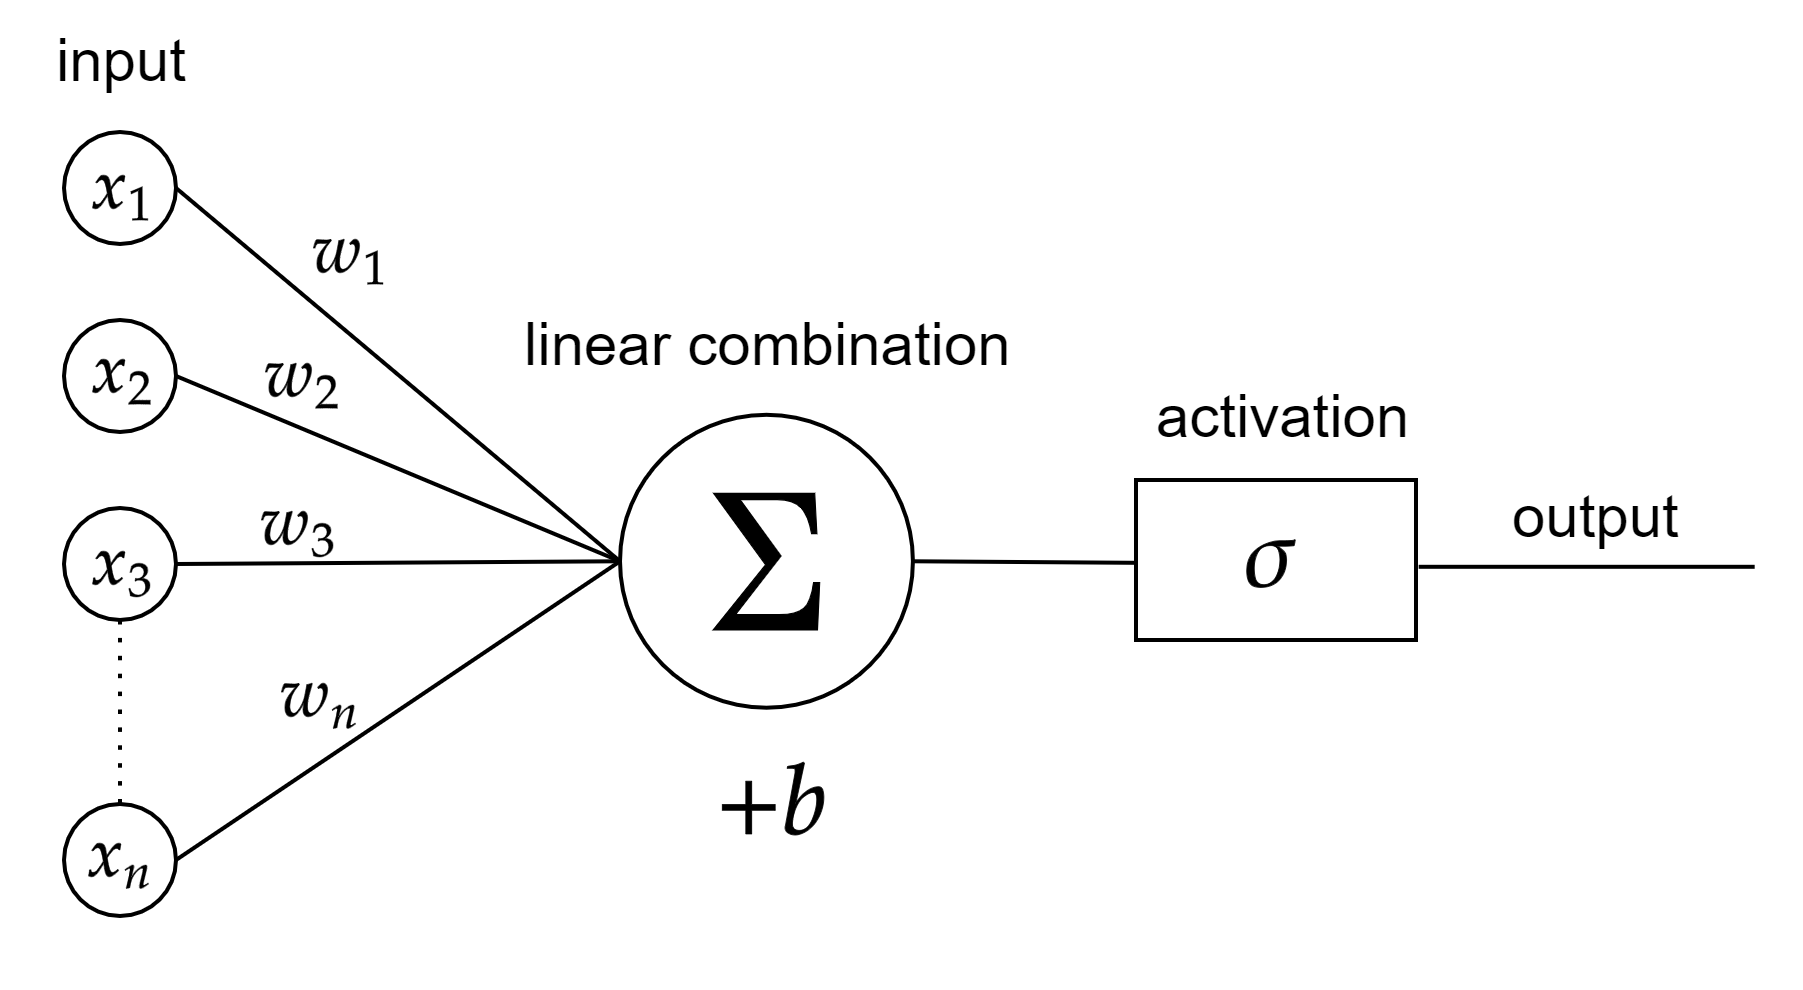
\includegraphics[scale=0.3]{img/diagram-20220205_1.png}
    \end{center}
    \caption{Illustration of the perceptron model for a single neuron.}
    \label{fig4}
\end{figure}

The choice of activation function is determined by the nature of the input and the assumed distribution of the output. When the activation function is for example equal to the Heaviside step function, i.e.
\begin{equation*}
    \sigma(x) = \begin{cases} 1 & \text{if } x \geq 0, \\ 0 & \text{if } x < 0, \end{cases}
\end{equation*}
then the perceptron coincides with a linear support vector classifier, see 
They are generally required to be monotone
increasing, continuous, and at least piecewise smooth. 
The non-linear functions used in neural networks include the rectified linear unit, commonly used in recent years, as well as the more conventional sigmoids, such as the hyberbolic tangent, 

At present, the most popular non-linear function is the rectified linear unit (ReLU), which is simply the half-wave rectifier. In past decades, neural nets used smoother non-linearities, such as , but the ReLU typically learns much faster in networks with many layers, allowing training of a deep supervised network without unsupervised pre-training28

\begin{align}
    \sigma(y) &=\tanh (y)=\frac{\exp (y)-\exp (-y)}{\exp (y)+\exp (-y)} & & \text { hyperbolic tangent } \\
    \sigma(y) &=\frac{1}{1+\exp (-y)} & & \text { logistic (soft step) } \\
    \sigma(y) &=\max \{y, 0\} & & \text { rectified linear unit (ReLU) } \\
    \sigma(y ; a) &=\max \{y, 0\}+\min \{a y, 0\} & & \text { parametric rectified linear unit (PReLU) } \\
    \sigma(y) &=\frac{y}{1+\exp (-y)} & & \text { swish function. }
\end{align}


After mentioning the XOR problem, which cannot be handled by perceptrons with one layer, we introduce multilayer perceptrons. 


Deep-learning methods are representation-learning methods with multiple levels of representation, obtained by composing simple but non-linear modules that each transform the representation at one level (starting with the raw input) into a representation at a higher, slightly more abstract level. With the composition of enough such transformations, very complex functions can be learned.

The most common form of machine learning, deep or not, is supervised learning.

The equations used for computing the forward pass in a neural net



The more complex the problem to be solved with the help of the neural network is, the more layers are needed. 

We compute an objective function that measures the error (or distance) between the output scores and the desired pattern of scores. The machine then modifies its internal adjustable parameters to reduce  this error. These adjustable parameters, often called weights, are real numbers that can be seen as ‘knobs’ that define the input–output function of the machine. In a typical deep-learning system, there may be hundreds of millions of these adjustable weights, and hundreds of millions of labelled examples with which to train the machine. To properly adjust the weight vector, the learning algorithm computes a gradient vector that, for each weight, indicates by what amount the error would increase or decrease if the weight were increased by a tiny amount. The weight vector is then adjusted in the opposite direction to the gradient vector. 

A deep-learning architecture is a multilayer stack of simple modules, all (or most) of which are subject to learning, and many of which compute non-linear input–output mappings. Each module in the stack transforms its input to increase both the selectivity and the invariance of the representation.

The backpropagation procedure to compute the gradient of an objective function with respect to the weights of a multilayer stack of modules is nothing more than a practical application of the chain rule for derivatives. The key insight is that the derivative (or gradient) of the objective with respect to the input of a module can be computed by working backwards from the gradient with respect to the output of that module

Many applications of deep learning use feedforward neural network architectures (Fig. 1), which learn to map a fixed-size input (for example, an image) to a fixed-size output (for example, a probability for each of several categories). To go from one layer to the next, a set of units compute a weighted sum of their inputs from the previous layer and pass the result through a non-linear function. At present, the most popular non-linear function is the rectified linear unit (ReLU), which is simply the half-wave rectifier. In past decades, neural nets used smoother non-linearities, such as , but the ReLU typically learns much faster in networks with many layers, allowing training of a deep supervised network without unsupervised pre-training28. Units that are not in the input or output layer are conventionally called hidden units. The hidden layers can be seen as distorting the input in a non-linear way so that categories become linearly separable by the last layer 

Perceptron
Activation Function
One layer
XOR Problem
Neural Network
FNN
%ResNet
Machine Learning, Training 
Supervised Learning
Unsupervised Learning
Gradient Based optimization
Backpropagation 
Honrik 